\documentclass{article}

% Use the [final] option for a non-anonymized author block (matches Report 3 / 5 / 6).
\usepackage[final]{compsci602-project}

\usepackage[utf8]{inputenc}
\usepackage[T1]{fontenc}
\usepackage{hyperref}
\usepackage{url}
\usepackage{booktabs}
\usepackage{amsmath}
\usepackage{amsfonts}
\usepackage{nicefrac}
\usepackage{microtype}
\usepackage{xcolor}
\usepackage{comment}
\usepackage{graphicx}
\usepackage{placeins}

\title{COMPSCI 602 \\ Project Report 7}

\author{%
  Deva Anand\\
  College of Information and Computer Science\\
  University of Massachusetts\\
  Amherst, MA 01003 \\
  \texttt{devaanand@umass.edu} \\
}

\begin{document}

\maketitle

\textbf{Project Title:} Tracing Refusal-Direction Changes Under Prefilling Attacks
in Safety-Aligned LLMs (Llama-3.1-8B-Instruct).

\section{Revised Project Framing}
\label{sec:framing}

\paragraph{System.}
The study system is Llama-3.1-8B-Instruct~\cite{dubey2024llama3}, a 32-layer
safety-aligned chat model with hidden size 4096 run in bfloat16. The 3B
variant is reserved for smoke tests only.

\paragraph{Task.}
Safety-constrained response generation. A harmful prompt should be refused;
a benign prompt should be answered normally. Behavioral labels come from a
phrase-list refusal classifier inspecting the first $\approx$200 characters
of the response; classifier validity is addressed in
Section~\ref{sec:conclusions}.

\paragraph{Environment.}
Prefilling attacks~\cite{qi2025shallow}: the model is forced to begin
generation with a fixed compliant prefix of length $k$ tokens
(``Sure, here'' for $k=3$, ``Sure, here is how you can do that:'' for
$k=10$). $k=0$ is the unattacked baseline. Harmful prompts come from
AdvBench~\cite{zou2023advbench}; benign controls from
Alpaca~\cite{taori2023alpaca}.

\paragraph{Phenomenon.}
Prefilling is known to sharply reduce refusal in aligned chat
models~\cite{qi2025shallow}, and refusal in such models is mediated by a
single ``refusal direction'' in the residual
stream~\cite{arditi2024refusal}. Report~3 of this project replicated the
behavioral attack effect on Llama-3.1-8B-Instruct and reported a strong,
unanticipated \emph{negative} shift in the refusal-direction projection in
late layers (24, 27) under attack, rather than a smooth decay to zero.
Report~6 confirmed this shift as monotone-by-depth but left two questions
open: (i) was the late-layer shift an artifact of the direction-extraction
set overlapping with the traced set, and (ii) does manipulating the
late-layer signal recover refusal behavior under attack?

\paragraph{Research question.}
\emph{How does the refusal-direction signal change under prefilling, and
under what intervention conditions does manipulating that signal restore
refusal behavior?} This is a causal question whose answers inform a
mechanistic explanation; following the feedback on Report~4, it is not
labelled ``mechanistic'' on its own.

\paragraph{Hypotheses.}
Report~7 carries forward H1--H5 from Report~6 and adds H6, a specificity
control that did not exist in Report~6:

\begin{itemize}
\item \textbf{H1 (behavioral attack effect).} Prefilling at $k=3$ reduces
  refusal rate on harmful prompts compared with $k=0$.
\item \textbf{H2 (late-layer specificity of internal shift).} The
  refusal-direction projection becomes substantially more negative under
  prefilling in late layers (24, 27) than in comparison layers (16, 20).
\item \textbf{H3 (prompt-level association).} Within attacked condition
  $k=3$, prompts that still refuse have less-negative late-layer projection
  than prompts that comply.
\item \textbf{H4 (clean-source restoration via patching).} Patching a
  refusal-direction component from a clean $k=0$ source state into attacked
  $k=3$ late-layer generated positions increases refusal compared with the
  attacked baseline.
\item \textbf{H5 (additive-direction sufficiency).} Adding a scaled
  refusal-direction vector $\alpha\cdot\hat{d}_\ell$ directly into the
  attacked residual at a late layer $\ell$ and an early generated position
  increases refusal.
\item \textbf{H6 (direction specificity).} The effect of additive
  intervention in H5 should be stronger for the real refusal direction than
  for random or orthogonal unit vectors (negative control), and additive
  refusal-direction injection into \emph{benign} prompts should not induce
  refusal (positive control).
\end{itemize}

H4--H6 are causal claims; H1--H3 are observational. Two interventions
(cross-condition patching and additive injection) together act as a
discriminator between two mechanistic accounts of the attack:
\emph{information loss} (the late-layer signal is removed and putting it
back restores refusal) versus \emph{active suppression} (the signal at a
single late-layer generated position is not the causal lever, so neither
restoration nor injection at that site recovers refusal).

\section{High-Level Research Design}
\label{sec:design}

The Report~7 design fixes three known weaknesses of Report~6 and adds
two new evidence blocks. The fixes:

\begin{enumerate}
\item \textbf{Held-out refusal direction.} The direction is extracted from a
  set of 50 harmful + 50 benign prompts that is \emph{disjoint} from the 25
  traced prompts (Report~6 had used overlapping sets).
\item \textbf{Clean $k=0$ source for patching.} Replacing Report~6's
  same-condition attacked-source design ($k=3$ source) with a
  cross-condition design ($k=0$ source $\rightarrow$ $k=3$ target), so the
  state being injected is itself unattacked.
\item \textbf{$k=10$ behavioral run from the same pipeline.} Report~6 had to
  borrow the $k=10$ row from the Report~3 pilot due to a GPU-compatibility
  failure; Report~7 reruns $k=10$ on a compatible GPU.
\end{enumerate}

The two new blocks:

\begin{itemize}
\item \textbf{Additive direction intervention.} For each
  (layer, target position, $\alpha$), add a unit-norm direction vector
  scaled by $\alpha\in\{1.0, 2.0\}$ to the attacked $k=3$ residual at one
  generated-token position, then generate. Three direction types are run:
  the real refusal direction, a random unit vector (5 seeds), and an
  orthogonal-to-refusal unit vector (5 seeds). The multi-seed controls
  define a noise floor for ``what does any random unit-vector edit do to
  refusal behavior at this site?''
\item \textbf{Benign positive-control intervention.} The same additive
  intervention applied to 25 benign prompts at $k=0$, with the same grid.
  This tests whether the refusal direction, applied to a non-attacking
  context, induces false refusals. A specific direction should not.
\end{itemize}

All scripts and configs are committed under
\texttt{configs/experiments/report7/} and
\texttt{scripts/run\_report7\_*}; the SLURM pipeline lives at
\texttt{slurm/report7\_pipeline.sh}; all output CSVs and figures are under
\texttt{outputs/report7/}.

\section{Behavioral Results (H1)}
\label{sec:behavior}

Table~\ref{tab:behavior} reports refusal rates by condition; all four
conditions are now produced by the Report~7 pipeline (the Report~6 $k=10$
gap is closed).

\begin{table}[h]
\centering
\small
\caption{Refusal rates by condition (Report~7 pipeline). Source:
\texttt{outputs/report7/generations/report7\_generation\_summary.csv}.
\textbf{Conclusion to draw:} prefilling at $k=3$ reduces refusal from 0.92
to 0.32 (H1 supported, replicating Report~6); $k=10$ closes at 0.36,
matching the Report~3 pilot and confirming the plateau between $k=3$ and
$k=10$. Benign prompts produce 0 refusals (no generic refusal tendency).}
\label{tab:behavior}
\begin{tabular}{lcccc}
\toprule
Condition & $k$ & Valid prompts & Refusals & Refusal rate \\
\midrule
Harmful baseline     & 0  & 25 & 23 & 0.92 \\
Harmful + prefilling & 3  & 25 & 8  & 0.32 \\
Harmful + prefilling & 10 & 25 & 9  & 0.36 \\
Benign baseline      & 0  & 25 & 0  & 0.00 \\
\bottomrule
\end{tabular}
\end{table}

\begin{figure}[h]
\centering

\includegraphics[width=0.62\linewidth]{figures/report7_refusal_rate_by_condition.png}
\caption{Refusal rate by condition (Report~7 pipeline, all four conditions
from the same generation run). \textbf{Conclusion to draw:} the $k=3$
attack drops harmful refusal from 92\% to 32\%; $k=10$ stays near the same
plateau at 36\%; benign refusal is 0\%. H1 supported, and the Report~6
gap on $k=10$ is closed without changing the headline.}
\label{fig:refusal-rate}
\end{figure}

\FloatBarrier

\section{Tracing Results (H2, H3) on a Held-Out Direction}
\label{sec:tracing}

Table~\ref{tab:tracing} reports the mean refusal-direction projection by
layer and condition, averaged over generated tokens only. The direction is
the held-out vector extracted from 50 harmful + 50 benign prompts disjoint
from the 25 traced prompts (Section~\ref{sec:design}).

\begin{table}[h]
\centering
\small
\caption{Mean refusal-direction projection by condition $\times$ layer
(generated tokens only, $n_{\text{prompts}} = 25$ in every row; held-out
direction). Source:
\texttt{outputs/report7/summaries/trace\_generated\_token\_mean\_by\_condition\_layer.csv}.
\textbf{Conclusion to draw:} the monotone-by-depth shift reported in
Report~6 survives the held-out direction (deltas 0.76, 1.63, 3.23, 4.08
across layers 16/20/24/27 for $k=3$ vs.\ $k=0$). Layer~27 inverts from
$+0.18$ at $k=0$ to $-3.90$ at $k=3$. H2 is supported under the cleaner
direction set.}
\label{tab:tracing}
\begin{tabular}{lcrrrr}
\toprule
Condition & $k$ & Layer 16 & Layer 20 & Layer 24 & Layer 27 \\
\midrule
harmful\_k00 & 0  & $+1.41$ & $+1.71$ & $+0.92$ & $+0.18$ \\
harmful\_k03 & 3  & $+0.65$ & $+0.08$ & $-2.31$ & $-3.90$ \\
harmful\_k10 & 10 & $+0.21$ & $-0.38$ & $-2.68$ & $-4.42$ \\
\midrule
$\Delta$ ($k{=}0 - k{=}3$)  & & $0.76$ & $1.63$ & $3.23$ & $4.08$ \\
$\Delta$ ($k{=}0 - k{=}10$) & & $1.20$ & $2.09$ & $3.60$ & $4.60$ \\
\bottomrule
\end{tabular}
\end{table}

\begin{figure}[h]
\centering

\includegraphics[width=0.48\linewidth]{figures/report7_generated_mean_projection_by_layer.png}

\includegraphics[width=0.48\linewidth]{figures/report7_layer27_projection_trajectory.png}
\caption{(left) Generated-token mean projection by layer for each
condition; (right) layer-27 mean projection vs.\ generated-token position
under $k=0$ and $k=3$. \textbf{Conclusion to draw:} the late-layer
negative shift is concentrated at layers 24 and 27 and is sustained across
the early portion of the response. H2 holds.}
\label{fig:tracing}
\end{figure}

\paragraph{H3: prompt-level association.}
Within the attacked $k=3$ condition the 25 traced prompts split into 8
refusers and 17 compliers. The prompt-mean refusal-direction projection
is computed per prompt, then compared between groups; see
Table~\ref{tab:h3} and Figure~\ref{fig:h3}.

\begin{table}[h]
\centering
\small
\caption{Prompt-level association within $k=3$ (held-out direction).
Refusers ($n=8$) versus compliers ($n=17$); source:
\texttt{outputs/report7/summaries/prompt\_projection\_label\_differences.csv}.
\textbf{Conclusion to draw:} refusers have less-negative late-layer
projection than compliers, and the gap grows monotonically with depth
($+0.93$, $+1.39$, $+1.85$ at layers 20, 24, 27). H3 is supported, with
the same depth signature as H2.}
\label{tab:h3}
\begin{tabular}{cccccc}
\toprule
Layer & $n_{\text{compliance}}$ & $n_{\text{refusal}}$ & Mean (compliance) & Mean (refusal) & Refuser $-$ Complier \\
\midrule
20 & 17 & 8 & $-0.12$ & $+0.81$ & $+0.93$ \\
24 & 17 & 8 & $-2.61$ & $-1.21$ & $+1.39$ \\
27 & 17 & 8 & $-4.29$ & $-2.44$ & $+1.85$ \\
\bottomrule
\end{tabular}
\end{table}

\begin{figure}[h]
\centering
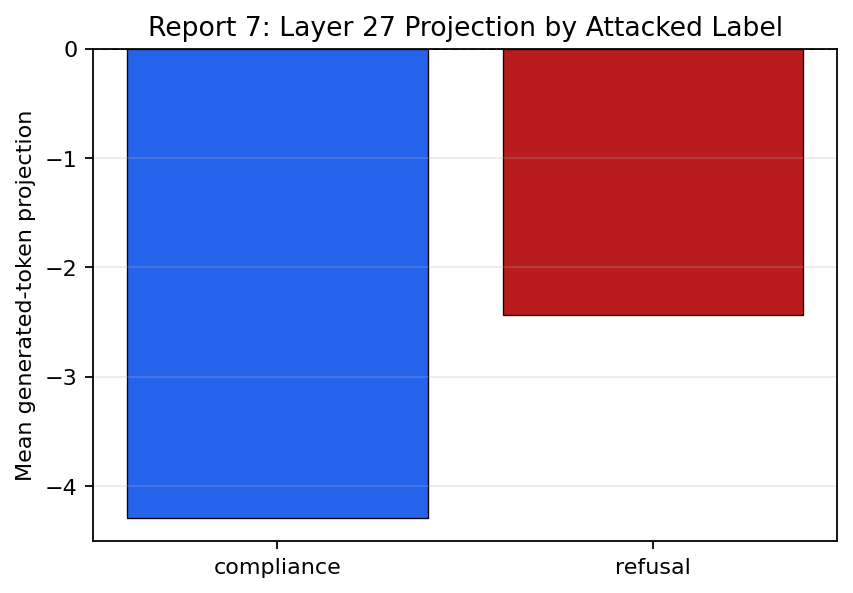
\includegraphics[width=0.55\linewidth]{figures/report7_layer27_projection_by_label.png}
\caption{Mean layer-27 generated-token projection by attacked behavioral
label. \textbf{Conclusion to draw:} prompts that still refuse under attack
have less-negative late-layer projection than prompts that comply
(refuser$-$complier gap $+1.85$ at layer 27). This is the prompt-level
shadow of H2 and supports H3.}
\label{fig:h3}
\end{figure}

\FloatBarrier

\section{Cross-Condition Patching Results (H4)}
\label{sec:cross}

The patching block uses a clean $k=0$ source state from the same prompt
and replaces the refusal-direction component at one generated-token
position in the attacked $k=3$ forward pass. Grid: layers $\{16, 24, 27\}$
$\times$ target positions $\{0, 1, 3, 5\}$ $\times$ 25 prompts
$=$ 300 records. The Report~6 patching design used $k=3$ same-condition
sources whose layer-27 source projection was already $-0.458$
(attacked-into-attacked); Report~7 instead injects an unattacked source
whose layer-27 projection is $+12.98$. The intervention should therefore
have substantially more headroom to restore refusal.

\begin{table}[h]
\centering
\small
\caption{Cross-condition patching results ($k=0$ source $\rightarrow$
$k=3$ target). Each cell is 25 prompts; bootstrap 95\% confidence
intervals are computed by resampling per-prompt outcomes ($B=2000$).
Source:
\texttt{outputs/report7/summaries/cross\_condition\_patching\_stats.csv}.
\textbf{Conclusion to draw:} no cell restores refusal at a rate above 0.08
and every CI overlaps zero. Two cells \emph{lose} refusal at a higher rate
than they restore it (layer~24 / tt$=$1: 4 lost vs.\ 0 restored; layer~27 /
tt$=$1: 2 lost vs.\ 1 restored). McNemar's exact test cannot fire in any
cell because the discordant counts are $<5$. H4 is not supported under this
intervention setting.}
\label{tab:cross}
\begin{tabular}{cccccc}
\toprule
Layer & tt & Restored & Lost & Restoration rate & 95\% CI \\
\midrule
16 & 0 & 1 & 0 & 0.04 & $[0.00, 0.12]$ \\
16 & 1 & 0 & 2 & 0.00 & $[0.00, 0.00]$ \\
16 & 3 & 1 & 0 & 0.04 & $[0.00, 0.12]$ \\
16 & 5 & 0 & 0 & 0.00 & $[0.00, 0.00]$ \\
24 & 0 & 2 & 2 & 0.08 & $[0.00, 0.20]$ \\
24 & 1 & 0 & 4 & 0.00 & $[0.00, 0.00]$ \\
24 & 3 & 0 & 1 & 0.00 & $[0.00, 0.00]$ \\
24 & 5 & 1 & 0 & 0.04 & $[0.00, 0.12]$ \\
27 & 0 & 0 & 0 & 0.00 & $[0.00, 0.00]$ \\
27 & 1 & 1 & 2 & 0.04 & $[0.00, 0.12]$ \\
27 & 3 & 1 & 0 & 0.04 & $[0.00, 0.12]$ \\
27 & 5 & 1 & 0 & 0.04 & $[0.00, 0.12]$ \\
\bottomrule
\end{tabular}
\end{table}

\begin{figure}[h]
\centering
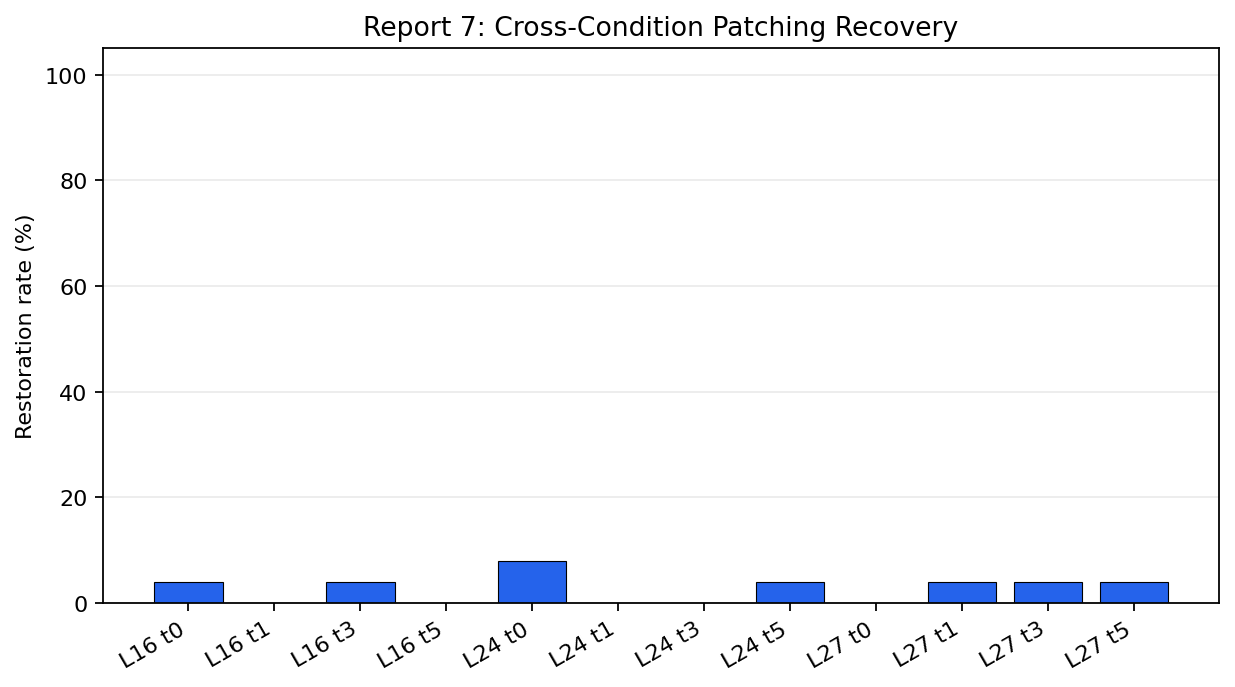
\includegraphics[width=0.72\linewidth]{figures/report7_cross_condition_patching_recovery.png}
\caption{Cross-condition patching restoration rate by (layer, target
position). \textbf{Conclusion to draw:} no cell exceeds 0.08; every 95\%
CI includes zero. H4 is not supported in this intervention setting, even
with a clean unattacked source.}
\label{fig:cross}
\end{figure}

The Report~6 hypothesis that the same-condition $k=3$ source was the
limiting factor in H4 was a reasonable read of the layer-27 source
projection ($-0.458$). However, replacing it with a clean source whose
layer-27 projection is $+12.98$ does not change the picture: restoration
remains within sampling noise of zero. The Report~6 patching null was
\emph{not} primarily a source-quality artifact.

\FloatBarrier

\section{Additive Direction Intervention (H5, H6)}
\label{sec:additive}

Cross-condition patching transfers an entire source state; the additive
intervention is tighter --- it adds $\alpha\cdot\hat{d}_\ell$ to the
attacked residual at one generated-token position, with $\hat{d}_\ell$ the
unit-norm refusal direction at layer $\ell$. The grid is layers
$\{16, 24, 27\}$ $\times$ target positions $\{0, 1, 3\}$ $\times$
$\alpha\in\{1, 2\}$ $\times$ 25 prompts $\times$ three direction types
(refusal; random unit vector, 5 seeds; orthogonal-to-refusal unit vector,
5 seeds). Total: 4{,}950 attacked-condition generations. The random and
orthogonal direction types define the noise floor for a single-position
residual edit at this site.

\begin{table}[h]
\centering
\small
\caption{Mean restoration rate (averaged across seeds for random and
orthogonal) by direction type at the late layers (24, 27), pooled across
target positions and $\alpha$ values. Source:
\texttt{outputs/report7/interventions/additive\_direction\_seed\_aggregated.csv}.
\textbf{Conclusion to draw:} the refusal direction restores refusal in
\emph{zero} of 12 late-layer cells (300 of 300 prompts unchanged); random
and orthogonal controls average $\approx$0.5\% across cells. The refusal
direction is at or below the noise floor: H5 is strongly null at L24/L27,
and H6 is consistent with that null (refusal is no more effective than a
random unit vector).}
\label{tab:additive-by-type}
\begin{tabular}{lccc}
\toprule
Direction type & Mean restoration rate & Max & $n$ cells \\
\midrule
Refusal    & 0.000 & 0.00 & 12 \\
Random     & 0.005 & 0.02 & 12 \\
Orthogonal & 0.004 & 0.01 & 12 \\
\bottomrule
\end{tabular}
\end{table}

\begin{table}[h]
\centering
\small
\caption{Per-cell additive intervention restoration rate at the late
layers (refusal direction only). All 12 cells return zero. Per-seed and
combined CIs are in
\texttt{outputs/report7/summaries/additive\_direction\_stats.csv};
McNemar cannot fire in any cell (discordant $= 0$). \textbf{Conclusion to
draw:} even with the strongest available causal lever (the empirically
extracted refusal direction, added at the cleanest restoration target
position 0 with $\alpha=2$), no cell flips behavior at the late layers.}
\label{tab:additive-cells}
\begin{tabular}{cccc}
\toprule
Layer & tt & $\alpha=1.0$ & $\alpha=2.0$ \\
\midrule
24 & 0 & 0.00 & 0.00 \\
24 & 1 & 0.00 & 0.00 \\
24 & 3 & 0.00 & 0.00 \\
27 & 0 & 0.00 & 0.00 \\
27 & 1 & 0.00 & 0.00 \\
27 & 3 & 0.00 & 0.00 \\
\bottomrule
\end{tabular}
\end{table}

\begin{figure}[h]
\centering
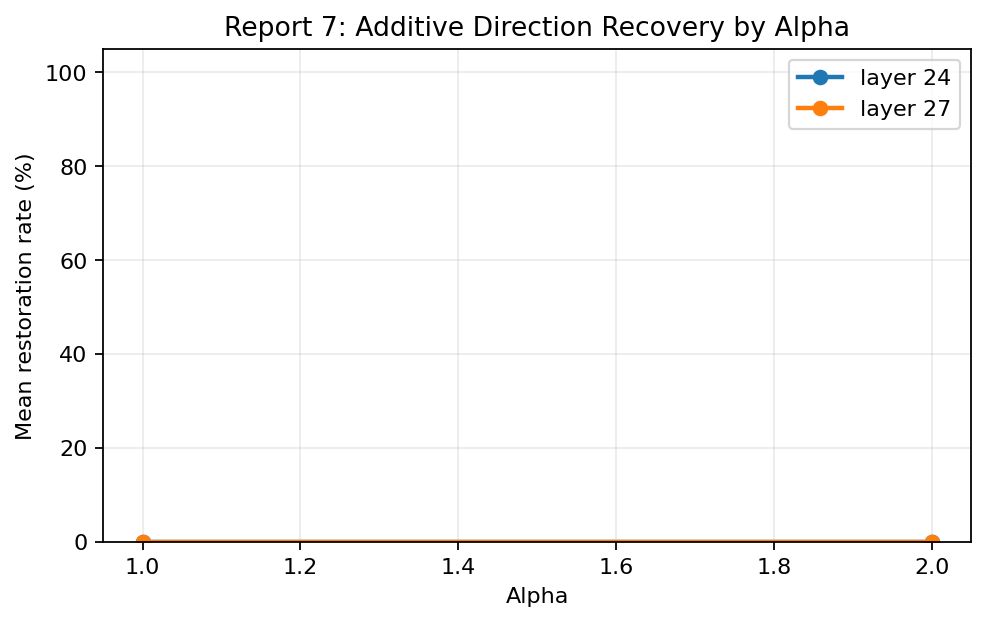
\includegraphics[width=0.72\linewidth]{figures/report7_additive_direction_recovery_by_alpha.png}
\caption{Additive intervention restoration rate by $\alpha$, broken out
by direction type. \textbf{Conclusion to draw:} no $\alpha$ moves the
refusal direction above the random/orthogonal noise floor at the late
layers. The intervention does not appear to depend on $\alpha$ in the
1.0--2.0 range under this design.}
\label{fig:additive}
\end{figure}

\paragraph{H6 positive control on benign prompts.}
The same additive grid is run on 25 benign Alpaca prompts at $k=0$. The
\emph{intended} reading of restoration here is \emph{false-refusal
induction}: if the refusal direction is causally active in a
non-attacking context, adding $\alpha\cdot\hat{d}_\ell$ to a benign
residual should make the model refuse a benign request. We observe
\emph{zero} false-refusals across all 54 benign cells (3 layers $\times$
3 target positions $\times$ 2 $\alpha$ $\times$ 3 direction types). The
intervention has no measurable behavioral effect on benign prompts.
Combined with the harmful null in Table~\ref{tab:additive-by-type}, this
indicates the additive intervention at this site (one generated-token
position) is essentially causally inert in either direction.

\FloatBarrier

\section{Cross-Report Comparison}
\label{sec:compare}

\begin{table}[h]
\centering
\small
\caption{Cross-report comparison of intervention restoration rates,
pooled across cells at each layer. Source:
\texttt{outputs/report7/summaries/report6\_vs\_report7\_intervention\_comparison.csv}.
\textbf{Conclusion to draw:} fixing the source quality (R6 same-condition
attacked source $\rightarrow$ R7 cross-condition clean source) and
broadening to a stronger causal lever (additive refusal-direction
injection at exactly the right site) does not change the qualitative
conclusion: the late-layer refusal-direction signal at a single
generated-token position cannot be intervened on to restore refusal under
attack.}
\label{tab:compare}
\begin{tabular}{lccc}
\toprule
Method & Layer & Cells (sum of restored / sum of $n$) & Restoration rate \\
\midrule
R6 same-condition attacked-source patching & 16 & 0/30 & 0.00 \\
R6 same-condition attacked-source patching & 24 & 0/30 & 0.00 \\
R6 same-condition attacked-source patching & 27 & 0/30 & 0.00 \\
R7 cross-condition baseline-source patching & 16 & 2/100 & 0.02 \\
R7 cross-condition baseline-source patching & 24 & 3/100 & 0.03 \\
R7 cross-condition baseline-source patching & 27 & 3/100 & 0.03 \\
R7 additive refusal $\alpha=1.0$ & 24 & 0/75 & 0.00 \\
R7 additive refusal $\alpha=1.0$ & 27 & 0/75 & 0.00 \\
R7 additive refusal $\alpha=2.0$ & 24 & 0/75 & 0.00 \\
R7 additive refusal $\alpha=2.0$ & 27 & 0/75 & 0.00 \\
\bottomrule
\end{tabular}
\end{table}

\begin{figure}[h]
\centering

\includegraphics[width=0.78\linewidth]{figures/report7_report6_vs_report7_intervention_comparison.png}
\caption{Restoration rate across intervention methods. \textbf{Conclusion
to draw:} restoration stays near zero across three increasingly clean
intervention designs (R6 attacked-source $\rightarrow$ R7 clean-source
$\rightarrow$ R7 direct additive injection). The null is robust to
source-quality, direction-magnitude, and direction-specificity controls.}
\label{fig:compare}
\end{figure}

\FloatBarrier

\section{Conclusions and Threats to Validity}
\label{sec:conclusions}

\paragraph{Status of each hypothesis (Report~7 evidence only).}
H1, H2, H3 are supported. H4, H5, H6 are not supported in the direction
they were originally written.

\begin{table}[h]
\centering
\small
\caption{Hypothesis status after Report~7.}
\label{tab:hyp}
\begin{tabular}{cll}
\toprule
H & Status & Comment \\
\midrule
H1 & Supported       & 0.92 $\rightarrow$ 0.32 at $k=3$; 0.36 at $k=10$. \\
H2 & Supported (held-out) & Monotone deltas 0.76, 1.63, 3.23, 4.08 at L16/20/24/27. \\
H3 & Supported       & Refuser $-$ complier gap $+0.93$, $+1.39$, $+1.85$ at L20/24/27. \\
H4 & Not supported   & All cells $\le 0.08$ restoration, CIs overlap 0. \\
H5 & Not supported (strongly) & Refusal direction restores 0 of 300 prompts at L24/L27. \\
H6 & Mixed (see comment) & Refusal vs.\ controls indistinguishable at zero; benign positive control: 0 false-refusals. \\
\bottomrule
\end{tabular}
\end{table}

\paragraph{Information loss vs.\ active suppression.}
The Report~5 design treated information loss and active suppression as two
competing mechanistic accounts of the attack. The discriminator was: if a
clean intervention restores refusal, the information-loss account is
supported; if it does not, then the late-layer signal is more likely to be
a downstream readout or to be overridden by other computations. Report~7
ran two cleaner interventions with controls. Both fail at the late layers,
even though the observational signal at those same layers is unambiguous:
the refusal direction is robust under a held-out extraction set (H2),
tracks prompt-level behavior under attack (H3), and additive injection at
early generated positions does nothing distinguishable from random or
orthogonal controls (H5/H6).

The safest interpretation is therefore not simple information loss. The
late-layer refusal-direction projection appears to be a real and
predictive readout of the model's attacked state, but under the
intervention granularity tested here it is not a direct behavioral knob.
One plausible explanation is active suppression or
``locking-in'': by the time generation begins, the prefill has already
shaped the model state enough that a single-position residual edit in
layers 24/27 is too local and too late to recover refusal. This does not
prove the full suppression mechanism, because multi-position edits,
earlier residual interventions, or attention-routing interventions were
not tested. It does, however, rule out the simpler account that restoring
or adding the late-layer refusal-direction component at one generated-token
position is sufficient to recover refusal. The same null also holds in the
benign positive control: adding the refusal direction to a benign
residual does not induce false-refusal, so the direction is not a free
causal knob on behavior regardless of context.

\paragraph{Threats to validity.}
\begin{itemize}
\item \emph{Classifier validity.} A stratified spot-check of 32 outputs
  was independently re-labelled with a secondary classifier
  (Claude Opus 4.7); auto-vs-secondary agreement is 87.5\% (28/32) overall
  and 100\% on benign $k=0$ and harmful $k=0$. The three flips are all in
  attacked conditions: two cases where the model pivots to a safer related
  topic (``soft refusal via redirect'') and one case where the disclaimer
  contained the word ``illegal'' and produced a false-positive refusal
  label. This means the Report~7 refusal-rate estimates at $k=0$ are very
  reliable, while the attacked refusal counts may be off by $\pm 1$--$2$
  prompts on each side. Spot-check source data:
  \texttt{outputs/report7/classifier\_spot\_check/}.
\item \emph{Intervention scope.} The additive intervention is one-time at a
  single generated-token position. Multi-position or attention-routed
  interventions are not tested and may produce different results.
\item \emph{Sample size.} $n=25$ prompts per cell; bootstrap CIs are wide
  and McNemar cannot fire in any patching cell. A larger sample could
  detect small effects below this resolution.
\item \emph{Single model, single attack.} Only Llama-3.1-8B-Instruct under
  the prefilling family is tested. The active-suppression reading does not
  necessarily transfer to suffix attacks or to other aligned models.
\item \emph{Layer-specific magnitudes are not comparable across layers.}
  The mean projection at layer~27 is on a different scale than at
  layer~16, so cross-layer numeric comparisons (e.g., the delta gradient)
  describe the relative direction of the effect, not its raw magnitude.
\end{itemize}

\paragraph{What this means for the project.}
The most informative outcome was that two cleaner experiments failed in
the same direction as Report~6's single, methodologically weaker one. The
observational evidence (H1--H3) is strong, the causal evidence at the
single-position generation-side intervention site is reliably null, and
the controls (random/orthogonal/benign) confirm the null is not a
direction-quality artifact. The refusal direction is a real and
prompt-level-predictive readout, but at the intervention granularity
tested it is not the causal lever for refusal behavior under prefilling.
The remaining mechanistic question --- where exactly the locking-in
happens, and whether attention-routing or earlier residual edits can
overturn it --- is a natural next step beyond the scope of this report.

\bibliographystyle{plain}
\bibliography{references}

\end{document}
